\section{Introduction}

\subsection{Motivation}

Dans un monde où les consommateurs sont de plus en plus conscients des implications éthiques, environnementales et sanitaires de leurs achats, il est crucial de fournir des outils qui permettent de faire des choix éclairés. L'application Ethiscan a été conçue pour répondre à ce besoin croissant. En scannant des produits, les utilisateurs peuvent obtenir des métadonnées détaillées et pertinentes sur ceux-ci. Ces informations permettent de savoir si un produit est local, équitable, biologique, ou répond à d'autres critères spécifiques que l'utilisateur juge importants. Ethiscan offre une solution moderne et pratique pour aligner les choix de consommation avec les valeurs personnelles des individus.

\subsection{Concept}

L'application Ethiscan se distingue par son approche innovante et personnalisée des métadonnées de produits. Contrairement à des applications existantes comme Yuka \cite{yuka}, qui se concentrent uniquement sur les métadonnées alimentaires, Ethiscan vise à créer une plateforme versatile où les utilisateurs peuvent s'abonner aux types de métadonnées qui leur importent le plus. Des mainteneurs spécialisés testent les produits et certifient les informations, assurant ainsi la fiabilité des données fournies. Cette plateforme unique ambitionne de rassembler une large base d'utilisateurs en leur offrant une solution intégrée et complète pour suivre les produits en fonction de leurs préférences et convictions personnelles. En facilitant l'accès à des informations détaillées et certifiées, Ethiscan se positionne comme un outil indispensable pour les consommateurs modernes et responsables.


\subsection{Vue d'ensemble des technologies}

Dans le développement de notre application mobile, nous avons adopté plusieurs technologies modernes pour garantir efficacité, performance et maintenabilité. Cette section présente une vue d'ensemble des technologies utilisées, organisées par front-end et back-end, ainsi que les outils de développement et de déploiement employés.

\begin{itemize}[noitemsep]
    \item \textbf{Framework principale :} Flutter
    \item \textbf{Versionnement et CI/CD :} GitHub, GitHub Actions
    \item \textbf{Authentification :} Firebase Authentication
    \item \textbf{Base de données :} Firebase Firestore
    \item \textbf{Scan de codes QR :} Librairie Google
    \item \textbf{Architecture :} Clean Architecture, Bloc
    \item \textbf{Automatisation de code :} JSON Serializable, Freezed
    \item \textbf{Localisation :} Localizations de base de Flutter
\end{itemize}

\subsection{Front-end}

Pour le développement de l'interface utilisateur, nous avons choisi Flutter comme framework principal. Flutter permet de créer des applications cross-platform, ce qui nous permet de cibler à la fois les utilisateurs Android et iOS avec une seule base de code. Voici quelques-unes des technologies et pratiques clés que nous avons utilisées pour le front-end :

\begin{itemize}[noitemsep]
    \item \textbf{Flutter :} Framework pour le développement d'interfaces utilisateur.
    \item \textbf{Bloc :} Utilisé pour la gestion de l'état, assurant une séparation claire des responsabilités et facilitant la testabilité.
    \item \textbf{I18n :} Pour supporter plusieurs langues et offrir une expérience utilisateur adaptée à différents marchés.
    \item \textbf{Google MlKit Barcode Scanning :} Intégrée pour offrir une fonctionnalité de scan rapide et précise.
\end{itemize}

\subsection{Technologies de Stockage}

Nous avons considéré différentes technologies pour stocker nos données avant de se tourner vers Firebase. Le tableau \ref{tab:technologies_stockage} récapitule les différentes technologies avec leurs caractéristiques clés :

\begin{table}[h!]
    \centering
    \resizebox{\textwidth}{!}{%
        \begin{tabular}{|c|c|c|c|c|c|c|}
            \hline
            \textbf{Technologie} & \textbf{Type} & \textbf{Scalabilité} & \textbf{Expérience} & \textbf{Services Complémentaires} & \textbf{Coûts} & \textbf{Cloud} \\
            \hline
            SQFLite              & SQL           & Limitée              & Faible              & Non                               & Gratuit        & Non            \\
            \hline
            Drift                & SQL           & Limitée              & Faible              & Non                               & Gratuit        & Non            \\
            \hline
            Firebase Firestore   & NoSQL         & Haute                & Élevée              & Authentification, Analytics       & Gratuit/Tier   & Oui            \\
            \hline
            Supabase             & NoSQL         & Haute                & Moyenne             & Authentification, API             & Variable       & Oui            \\
            \hline
            Flutter Storage      & NoSQL         & Limitée              & Moyenne             & Non                               & Gratuit        & Non            \\
            \hline
            Hive                 & NoSQL         & Limitée              & Faible              & Non                               & Gratuit        & Non            \\
            \hline
            ObjectBox            & NoSQL         & Haute                & Faible              & Sync, GraphQL API                 & Variable       & Oui            \\
            \hline
            Shared Preferences   & NoSQL         & Limitée              & Moyenne             & Non                               & Gratuit        & Non            \\
            \hline
        \end{tabular}
    }
    \caption{Comparatif des technologies de stockage pour Flutter}
    \label{tab:technologies_stockage}
\end{table}

\subsubsection{Choix de Technologie}
Nous avons choisi Firebase Firestore pour plusieurs raisons clés. En tant que base de données NoSQL, elle élimine l'impedance mismatch, simplifiant ainsi le développement. Firebase est gratuit dans son tier initial, ce qui est idéal pour démarrer sans coûts initiaux. Étant basé dans le cloud, il permet une synchronisation en temps réel des données. De plus, Firebase offre des services intégrés tels que l'authentification et les analytics, réduisant ainsi le besoin de solutions tierces. L'expérience préalable d'un membre de notre équipe avec cette technologie a également été un atout majeur. En somme, Firebase Firestore s'est avéré être la solution idéale, offrant une intégration simplifiée, des coûts initiaux réduits, des services complets, et une accélération du développement sans nécessiter de backend complexe.


\subsection{Méthodologie de Développement}

\subsubsection{Kanban}

Les tâches sont organisées en issues avec les états suivants :

\begin{itemize}[noitemsep]
    \item \textbf{To Do} : Tâches dont l'implémentation n'est pas encore commencée. Elles peuvent cependant déjà être attribuées.
    \item \textbf{In Progress} : Tâches en cours d'implémentation.
    \item \textbf{To Review} : Une fois l'implémentation terminée, le développeur ouvre une pull request et place la story dans cette colonne. Un autre développeur vérifie l'implémentation, peut laisser des commentaires, et s'assigne la story en tant que reviewer. Si l'implémentation nécessite des modifications, il la déplace dans la colonne "To Do" avec des commentaires explicatifs. Sinon, il ferme la pull request et déplace l'issue dans "Done".
    \item \textbf{Done} : Tâches terminées.
\end{itemize}

\subsubsection{Outils de développement}

Pour assurer une gestion efficace du projet et maintenir une haute qualité de code, nous avons utilisé les outils suivants :

\begin{itemize}[noitemsep]
    \item \textbf{GitHub :} Plateforme de gestion de code source, facilitant la collaboration entre les membres de l'équipe.
    \item \textbf{GitHub Actions :} Utilisé pour automatiser le processus de compilation à chaque push de code, et pour exécuter des linters afin de maintenir la cohérence et la qualité du code.
    \item \textbf{JSON Serializable et Freezed :} Paquets utilisés pour l'automatisation de la sérialisation des objets JSON, réduisant les erreurs manuelles et accélérant le développement.
\end{itemize}

\subsection{Architecture}
\label{sec:architecture}

Pour garantir la robustesse et la maintenabilité de notre application Flutter, nous avons adopté le principe de la Clean Architecture \cite{cleanArchitecture}. Ce paradigme architectural permet une séparation claire des responsabilités, divisant le projet en plusieurs couches distinctes :

\begin{itemize}[noitemsep]
    \item \textbf{Domain Layer} : Cette couche contient la logique métier et les entités de l'application. Elle est indépendante des détails d'implémentation et des frameworks, ce qui facilite les tests unitaires et la réutilisation du code.
    \item \textbf{Data Layer} : Responsable de la gestion des sources de données (API, bases de données locales, etc.), cette couche implémente les interfaces définies dans la couche Domain. Elle assure également la conversion des données entre les formats utilisés par les sources externes et les entités du domaine.
    \item \textbf{Repository Layer} : Les repositories servent d'intermédiaires entre la couche Domain et la couche Data. Ils encapsulent la logique de récupération et de persistance des données, offrant une interface simplifiée pour les use cases de l'application.
    \item \textbf{Presentation Layer} : Cette couche gère l'interface utilisateur et les interactions. Elle utilise les données fournies par les use cases pour mettre à jour l'état de l'interface.
\end{itemize}

En plus de la Clean Architecture, nous avons implémenté le pattern Bloc (Business Logic Component) pour la gestion des états \cite{blocPattern}. Le pattern Bloc facilite la séparation entre la logique de présentation et la logique métier, en utilisant des flux de données réactifs (Streams). Chaque Bloc gère un état spécifique de l'application et réagit aux événements émis par l'interface utilisateur pour produire de nouveaux états.

La combinaison de la Clean Architecture et du pattern Bloc nous a permis de concevoir une architecture modulaire, testable et évolutive. Cette approche nous a permis de créer une application à la fois robuste et professionnelle, répondant aux exigences de qualité nécessaires pour un projet de cette envergure.


\begin{figure}[H]
    \centering
    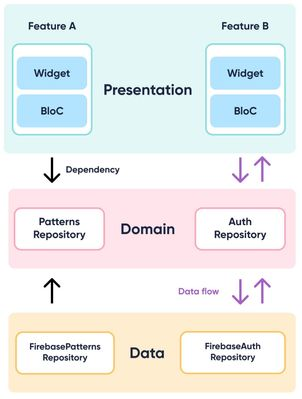
\includegraphics[width=0.5\textwidth]{images/firebase-architecture-BLoC.jpeg}
    \caption{Clean Architecture et BLoC pour la structure de l'application. (image récupérée sur \cite{googleCloudArchitecture})
    }
    \label{fig:architecture}
\end{figure}


%Des mainteneurs spécialisés testent les produits et certifient les informations, assurant ainsi la fiabilité des données fournies